% 第5章 本研究の特徴
\newpage
\renewcommand{\baselinestretch}{1.5}
\section{本研究の特徴}
\renewcommand{\baselinestretch}{1}
\par 本研究の特徴は既存の顕著性マップ生成モデルとウェブページの構造を組合せる事で、ウェブページのレイアウトを考慮して要素単位での顕著度を正確に予測するということである。要素単位の顕著度を正確に予測するためにウェブページ閲覧時の視線データセットを作成した。計算した顕著度を用いて、ピクセル単位ではなく要素単位での顕著性を視覚化して顕著領域マップの生成を行う。また、要素の顕著度ランキングを計算して顕著度が高い領域をトリミングすることで重要度の高い領域を視覚化する集約図の生成を行う。

\subsection{視線データセットの作成}
\par 人間の注視はボトムアップ要因とトップダウン要因の二種類の特徴を組み合わせて処理を行う。ボトムアップ要因とは輝度特性や色特性や方向特性などで、周囲の刺激と顕著に異なる場合に注意が引き付けられる。一方でトップダウン要因とは事前知識などがある際にそれらに基づいて能動的にバイアスがかかり注意が引き付けられることを示す。風景などの自然画像と比較してウェブページには写真やテキストやロゴなどの固有の要素が多数存在していてこれらが正確な顕著性の予測を困難にしている。Shenら\cite{shen2014webpage}の人間の視線を測定するアイトラッカーを用いてウェブページの顕著性を測定した実験によると、図\ref{fig_shen-experience}に示すようにテキスト中心と画像中心とテキスト画像が混合した全てのウェブページにおいて人は左上の領域と中心付近に目線が行く傾向が判明した。ウェブページの左上から中央にかけての領域に注目が集まるの現象はf-biasと言う名で一般的に知られており、このようにバイアスを考慮して正確な顕著性を予測するためにユーザーがウェブページを閲覧する際の視線データが必要となる。しかしながら、ウェブ上に公開されている視線のデータセットはほとんど存在しておらず、近年のモダンデザインに対応しているものは存在しないためオリジナルデータセットを作成する。

\begin{figure}[H]
  \centering
  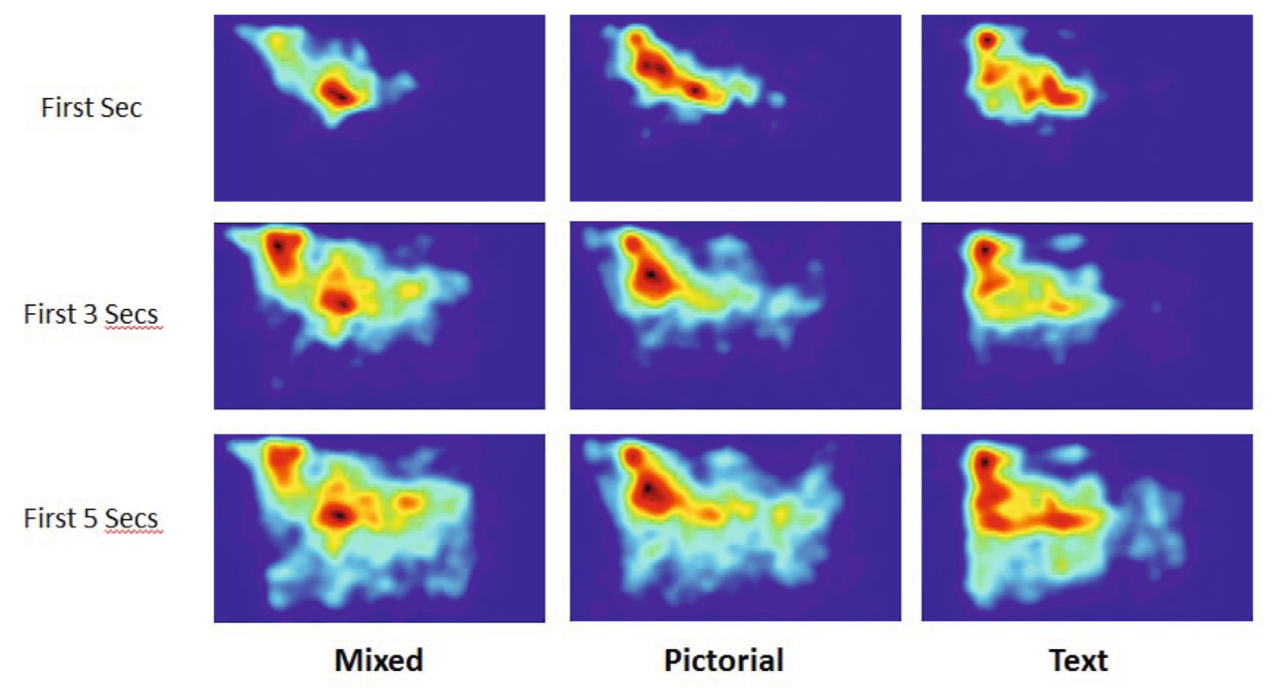
\includegraphics[width=8cm]{figures/shen-bias.png}
  \caption{Shenらのウェブページのヒートマップ生成実験結果\cite{shen2014webpage}}
  \label{fig_shen-experience}
\end{figure}

\subsection{要素単位での顕著性マップの生成}
\par 通常の顕著性マップではグレースケールで顕著性を表現するが、これだけではどの領域が重要度が高いであろうというざっくりとした予想しか行う事ができない。ウェブページを閲覧する際に人は、画像やタイトルやリンクなどタグ単位の要素で重要度を判断する事が多い。そこで本研究では要素単位の顕著性を計算してランキング付けをする事で、正確にどの要素の顕著性が高いのか判断できるウェブページに特化した要素単位の顕著領域マップを生成する事が効果的だと考えた。図\ref{fig_comparesaliency}に早稲田大学ウェブサイトトップページ(2018年12月時点)\cite{waseda_top}のスクリーンショットを入力した時に生成される既存の顕著性マップと提案手法の顕著領域マップの比較を示す。なお、提案手法の顕著領域マップ上の緑色の枠線は特に顕著度が高い重要領域10箇所を表している。

\begin{figure}[H]
    \centering
    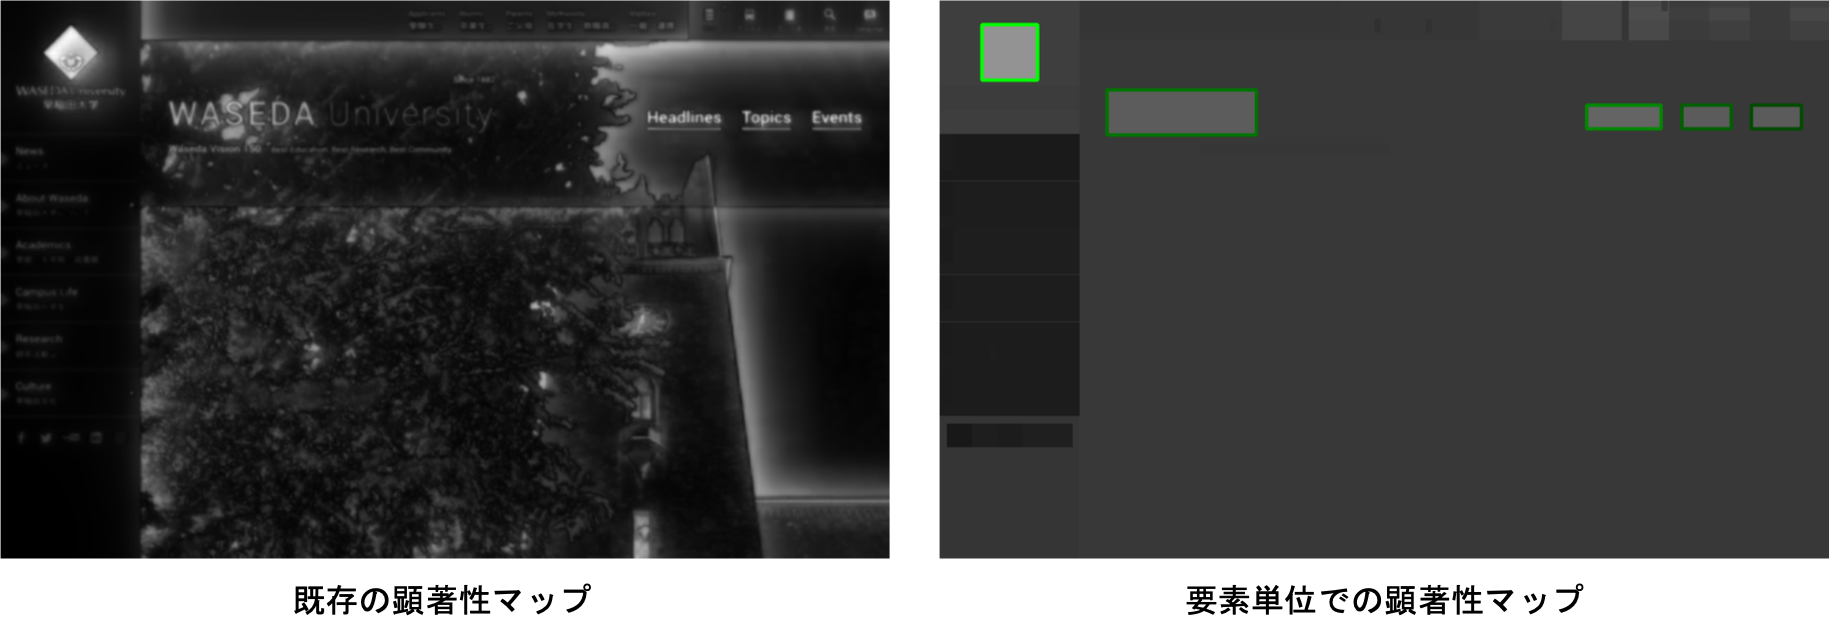
\includegraphics[width=12cm]{figures/example-originalsaliencymap.png}
    \caption{既存の顕著性マップと要素単位での顕著性マップとの比較}
    \label{fig_comparesaliency}
\end{figure}

\subsection{重要領域の視覚化}
\par ウェブページの顕著領域にはウェブページの重要な内容が含まれる事が多い。既存の研究では精度の高い顕著性マップの生成を行う事で研究が完結している事がほとんどである。しかしながら、要素ごとの顕著性を計算する事で作成した顕著度ランキングを元に重要領域ををタイル状に並べて一つの画像にまとめる事でウェブページの内容を簡単に把握可能な集約図を生成出来ると考えた。これにより、ネットユーザーが初見のウェブページにアクセスした際の内容把握の時間短縮に繋がる可能性がある。図\ref{fig_imoortanceregion}に早稲田大学ウェブサイトトップページ(2018年12月時点)\cite{waseda_top}の重要領域を集約した集約図を示す。

\begin{figure}[H]
    \centering
    
\includegraphics[width=8cm]{figures/example-importanceregion.png}
    \caption{生成された集約図の例}
    \label{fig_imoortanceregion}
\end{figure}
